\begin{equation}
    \begin{gathered}
        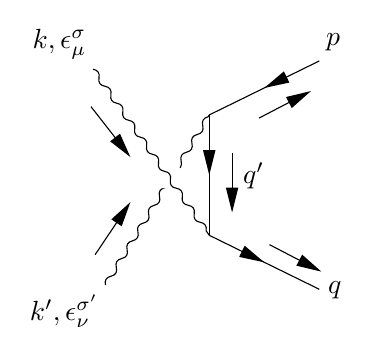
\begin{tikzpicture}[x=0.75pt,y=0.75pt,yscale=-1,xscale=1]
            %uncomment if require: \path (0,300); %set diagram left start at 0, and has height of 300
            
            %Straight Lines [id:da3057302086045661] 
            \draw    (152,184.67) .. controls (151.45,182.38) and (152.31,180.95) .. (154.6,180.4) .. controls (156.89,179.85) and (157.76,178.42) .. (157.21,176.13) .. controls (156.65,173.84) and (157.52,172.41) .. (159.81,171.86) .. controls (162.1,171.31) and (162.97,169.88) .. (162.41,167.59) .. controls (161.86,165.3) and (162.73,163.87) .. (165.02,163.32) .. controls (167.31,162.77) and (168.18,161.34) .. (167.62,159.05) .. controls (167.06,156.76) and (167.93,155.33) .. (170.22,154.78) .. controls (172.51,154.23) and (173.38,152.8) .. (172.82,150.51) .. controls (172.27,148.22) and (173.14,146.8) .. (175.43,146.25) .. controls (177.72,145.7) and (178.59,144.27) .. (178.03,141.98) .. controls (177.47,139.69) and (178.34,138.26) .. (180.63,137.71) .. controls (182.92,137.16) and (183.79,135.73) .. (183.24,133.44) .. controls (182.68,131.15) and (183.55,129.72) .. (185.84,129.17) .. controls (188.13,128.62) and (189,127.19) .. (188.44,124.9) .. controls (187.89,122.61) and (188.76,121.18) .. (191.05,120.63) .. controls (193.34,120.08) and (194.21,118.65) .. (193.65,116.36) .. controls (193.09,114.07) and (193.96,112.64) .. (196.25,112.09) .. controls (198.54,111.54) and (199.4,110.12) .. (198.85,107.83) .. controls (198.3,105.54) and (199.17,104.11) .. (201.46,103.56) -- (202,102.67) -- (202,102.67) ;
            %Shape: Circle [id:dp7275452294524412] 
            \draw  [draw opacity=0][fill={rgb, 255:red, 255; green, 255; blue, 255 }  ,fill opacity=1 ] (172,130) .. controls (172,125.58) and (175.58,122) .. (180,122) .. controls (184.42,122) and (188,125.58) .. (188,130) .. controls (188,134.42) and (184.42,138) .. (180,138) .. controls (175.58,138) and (172,134.42) .. (172,130) -- cycle ;
            %Straight Lines [id:da9256849462699361] 
            \draw    (255,76.67) -- (202,102.67) ;
            \draw [shift={(228.5,89.67)}, rotate = 333.87] [fill={rgb, 255:red, 0; green, 0; blue, 0 }  ][line width=0.08]  [draw opacity=0] (12,-3) -- (0,0) -- (12,3) -- cycle    ;
            %Straight Lines [id:da488527311343778] 
            \draw    (202,102.67) -- (202,160.67) ;
            \draw [shift={(202,131.67)}, rotate = 270] [fill={rgb, 255:red, 0; green, 0; blue, 0 }  ][line width=0.08]  [draw opacity=0] (12,-3) -- (0,0) -- (12,3) -- cycle    ;
            %Straight Lines [id:da2615197234092139] 
            \draw    (146,80.67) .. controls (148.32,81.08) and (149.28,82.44) .. (148.87,84.76) .. controls (148.46,87.08) and (149.41,88.45) .. (151.73,88.86) .. controls (154.05,89.27) and (155.01,90.64) .. (154.6,92.96) .. controls (154.19,95.28) and (155.15,96.64) .. (157.47,97.05) .. controls (159.79,97.46) and (160.75,98.83) .. (160.34,101.15) .. controls (159.93,103.47) and (160.88,104.83) .. (163.2,105.24) .. controls (165.52,105.65) and (166.48,107.02) .. (166.07,109.34) .. controls (165.66,111.66) and (166.62,113.03) .. (168.94,113.44) .. controls (171.26,113.85) and (172.22,115.21) .. (171.81,117.53) .. controls (171.4,119.85) and (172.35,121.22) .. (174.67,121.63) .. controls (176.99,122.04) and (177.95,123.4) .. (177.54,125.72) .. controls (177.13,128.04) and (178.09,129.41) .. (180.41,129.82) .. controls (182.73,130.23) and (183.69,131.6) .. (183.28,133.92) .. controls (182.87,136.24) and (183.82,137.6) .. (186.14,138.01) .. controls (188.46,138.42) and (189.42,139.79) .. (189.01,142.11) .. controls (188.6,144.43) and (189.56,145.8) .. (191.88,146.21) .. controls (194.2,146.62) and (195.15,147.98) .. (194.74,150.3) .. controls (194.33,152.62) and (195.29,153.99) .. (197.61,154.4) .. controls (199.93,154.81) and (200.89,156.17) .. (200.48,158.49) -- (202,160.67) -- (202,160.67) ;
            %Straight Lines [id:da7955957386194441] 
            \draw    (255,186.67) -- (202,160.67) ;
            \draw [shift={(228.5,173.67)}, rotate = 206.13] [fill={rgb, 255:red, 0; green, 0; blue, 0 }  ][line width=0.08]  [draw opacity=0] (12,-3) -- (0,0) -- (12,3) -- cycle    ;
            %Straight Lines [id:da8700765164776401] 
            \draw    (145,98.67) -- (162.77,121.42) ;
            \draw [shift={(164,123)}, rotate = 232.02] [fill={rgb, 255:red, 0; green, 0; blue, 0 }  ][line width=0.08]  [draw opacity=0] (12,-3) -- (0,0) -- (12,3) -- cycle    ;
            %Straight Lines [id:da7164688914224506] 
            \draw    (147,170) -- (162.89,146.33) ;
            \draw [shift={(164,144.67)}, rotate = 123.86] [fill={rgb, 255:red, 0; green, 0; blue, 0 }  ][line width=0.08]  [draw opacity=0] (12,-3) -- (0,0) -- (12,3) -- cycle    ;
            %Straight Lines [id:da4544265427173353] 
            \draw    (249.23,92.09) -- (226,104.17) ;
            \draw [shift={(251,91.17)}, rotate = 152.53] [fill={rgb, 255:red, 0; green, 0; blue, 0 }  ][line width=0.08]  [draw opacity=0] (12,-3) -- (0,0) -- (12,3) -- cycle    ;
            %Straight Lines [id:da7941011992391758] 
            \draw    (254.23,177.24) -- (231,165.17) ;
            \draw [shift={(256,178.17)}, rotate = 207.47] [fill={rgb, 255:red, 0; green, 0; blue, 0 }  ][line width=0.08]  [draw opacity=0] (12,-3) -- (0,0) -- (12,3) -- cycle    ;
            %Straight Lines [id:da44874471775014224] 
            \draw    (213,121) -- (213,147.67) ;
            \draw [shift={(213,149.67)}, rotate = 270] [fill={rgb, 255:red, 0; green, 0; blue, 0 }  ][line width=0.08]  [draw opacity=0] (12,-3) -- (0,0) -- (12,3) -- cycle    ;
            
            % Text Node
            \draw (257,73.27) node [anchor=south west] [inner sep=0.75pt]    {$p$};
            % Text Node
            \draw (258,181.57) node [anchor=north west][inner sep=0.75pt]    {$q$};
            % Text Node
            \draw (217,124.4) node [anchor=north west][inner sep=0.75pt]    {$q'$};
            % Text Node
            \draw (144,77.27) node [anchor=south east] [inner sep=0.75pt]    {$k,\epsilon _{\mu }^{\sigma }$};
            % Text Node
            \draw (150,188.07) node [anchor=north east] [inner sep=0.75pt]    {$k',\epsilon _{\nu }^{\sigma '}$};
            \end{tikzpicture}            
    \end{gathered} 
    \begin{aligned}[t]
        &= \epsilon^\sigma_\mu \epsilon^{\sigma'}_\nu \times \ii e (p - (q-k))^\nu \times \ii e (- q - (q-k))^\mu \times \frac{\ii}{(q-k)^2 - m^2 + \ii 0^+} \\
        &= \ii e^2 \epsilon^\sigma_\mu (2q-k)^\mu \epsilon^{\sigma'}_\nu (p-q+k)^\nu \frac{1}{(q-k)^2 - m^2 + \ii 0^+} \eqqcolon \ii \mathcal{M}_u.
    \end{aligned}
\end{equation}